\documentclass{beamer}
\usepackage{ru}
\usepackage[export]{adjustbox}

\title{The Speed of Heat}
\subtitle{in collaboration with Alliander}
\author{Erik Mulders}
\institute{Radboud University Nijmegen}
\date{12\textsuperscript{th} April 2022}

\begin{document}
	
	\frame{\titlepage}
	
	\begin{frame}{About Alliander}
		% Spreekt redelijk voor zich, een korte intro over Alliander als bedrijf
		% Het is me niet geheel duidelijk hoe Alliander nou in elkaar steekt, dit is een deel van wat ik kon vinden
		% Voel je vrij om hier nog aan toe te voegen
		\begin{columns}[T]
			\begin{column}{0.5\linewidth}
				\begin{itemize}
					\item Liander: distribution network operator (DNO)
					\begin{itemize}
						\item Active in 5 provinces $\rightarrow$
					\end{itemize}
					\item Qirion: high voltage network
				\end{itemize}
			\end{column}
			\begin{column}{0.5\linewidth}
				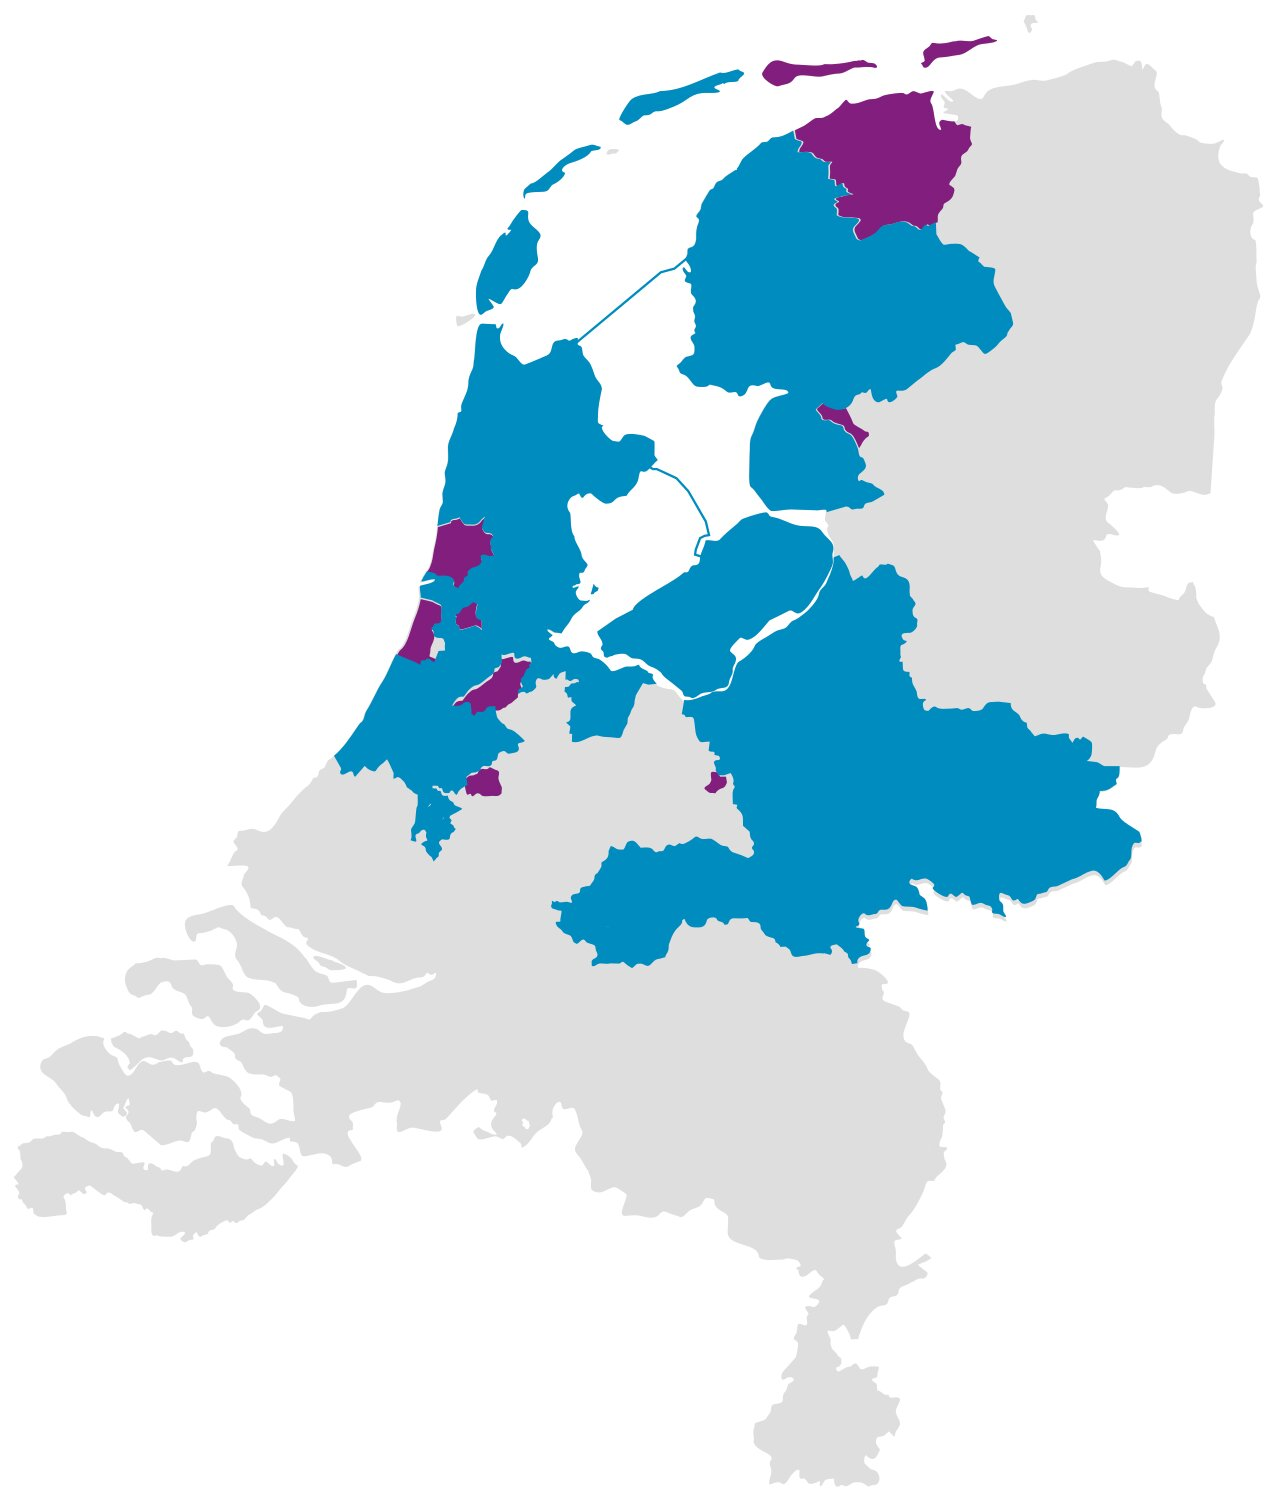
\includegraphics[width=\linewidth]{liander-in-kaart}
				% Blauw is elektriciteit én gas, paars alleen elektriciteit
				% Bron: https://www.liander.nl/over-liander/werkgebied
			\end{column}
		\end{columns}
	\end{frame}
	
	\begin{frame}{Smart Cable Guard}
		% Hier iets over hoe SCG werkt en dat er vaak lange stukken kabel tussen twee meetpunten zitten -> onzekerheid in waarden tussen meetpunten, interpolatie is nodig
		% Introduceer de verschillende typen kabel (PILC/XLPE)
	\end{frame}
	
	\begin{frame}{Cable temperature and partial discharges}
		% Hier iets over waarom de kabeltemperatuur belangrijk is en wat PD's zijn en dat de twee concepten gerelateerd zijn
	\end{frame}
	
	\begin{frame}{How to determine the cable temperature}
		% Hier iets over de verschillende modellen die aangedragen zijn
		% Ook kort iets over hoe de modellen tot stand komen (e.g. heat equation, formule voor propagatiesnelheid in termen van permittiviteit)
		$$T_\text{cable} = C I^2 + T_\text{ground}$$
		~\\
		$$T_\text{cable} = \alpha_1 P(t) + \alpha_0$$
	\end{frame}
	
	\begin{frame}{Research question}
		% Beschrijving van de 4 vragen die in de repo staan
		\footnotesize
		% Deze \footnotesize hierboven kan weg als je de vragen iets inkort
		\begin{enumerate}
			\item In cases where the load on the cable is sufficiently low, we can assume that the cable is always at soil temperature. In particular the correlation between soil temperature and propagation time will be very high. How can we recognize such cases quickly?
			\item Suppose we assume a very simple model for cable temperature, for example $T_\text{cable}(t) = C P(t) + T_\text{soil}$ where $I(t)$ is the current through the cable and $C$ is a constant. What can you say about the error (bias and variance) of this model? Is this model realistic? Can you propose an improvement?
			\item Can you propose a method to estimate the model uncertainty of the temperature estimate? A method that seems promising is Bayesian linear regression, which yields a confidence interval around models estimates.
			\item Smart Cable Guard measures noise, expressed as a sensitivity time series. This is likely to affect the accuracy of the propagation time measurement. Can you show this from the data? How does the error $\varepsilon(t)$ depend on the sensitivity?
		\end{enumerate}
	\end{frame}
	
	\begin{frame}{Our progress so far: question 2}
		% Wat hebben we al gedaan met vraagstuk nummer 2?
		% Volgens Arthur en Gabriël: er is een (voor zover) werkende Python class gemaakt die een model voorstelt, en deze moet nog geïntegreerd worden in de rest van de code
	\end{frame}
	
	\begin{frame}{Our progress so far: question 3}
		% Wat hebben we al gedaan met vraagstuk nummer 3?
		% Volgens Gabriël: Vraag 3 heeft een (zover hij weet) werkende functie om de betrouwbaarheid uit te rekenen met bayesian linear regression
	\end{frame}
	
	\begin{frame}{What's next?}
		% Hier iets over de korte- en langetermijndoelen
		% Daar hoort natuurlijk bij dat we aandacht besteden aan vraag 1 en 4 
		\begin{itemize}
			\item 
			\item 
			\item 
			\item 
			\item 
		\end{itemize}
	\end{frame}
\end{document}